\documentclass[border=3pt]{standalone}
% Preâmbulo compartilhado pelos diagramas TikZ da aula 4 de Navegação (Representação de Mapas)
\usepackage[T1]{fontenc}
\usepackage[utf8]{inputenc}
\usepackage{lmodern}
\usepackage{amsmath}
\usepackage{xcolor}
\usepackage{tikz}
\usetikzlibrary{arrows.meta,angles,quotes,decorations.pathmorphing,decorations.pathreplacing,calc,
                positioning,shapes.geometric,shapes.misc,backgrounds,fit,
                math}

% Paleta (mesma dos SVGs originais)
\definecolor{dblue}{HTML}{2A5B8C}
\definecolor{dorange}{HTML}{B3541E}
\definecolor{dgreen}{HTML}{4A7C59}
\definecolor{dred}{HTML}{9C4B4B}
\definecolor{dcream}{HTML}{F4F1EA}
\definecolor{dshade}{HTML}{DDD7C9}

% Função gaussiana (não normalizada por padrão de escala visual)
\pgfmathdeclarefunction{gauss}{3}{%
  \pgfmathparse{1/(#3*sqrt(2*pi))*exp(-((#1-#2)^2)/(2*#3^2))}%
}

% Estilos comuns (prefixo d... para não colidir com chaves internas do pgf)
\tikzset{
  >={Stealth[length=2mm]},
  dguide/.style={gray!55, dashed, line width=0.4pt},
  daxis/.style={gray!60, line width=0.7pt, ->},
  dbody/.style={fill=black!3, draw=black!80, line width=1pt},
  dacc/.style={draw=dblue, line width=1pt},
  dlbl/.style={black!55, font=\small},
  dsub/.style={black!45, font=\footnotesize},
  dstate/.style={circle, draw=black!80, fill=dcream, line width=1pt,
                 minimum size=17mm, font=\large, inner sep=1pt},
  dobs/.style={circle, draw=black!80, fill=dshade, line width=1pt,
               minimum size=14mm, font=\large, inner sep=1pt},
  dbox/.style={rounded corners=2pt, draw=black!80, fill=dcream, line width=1pt,
               align=center, inner sep=6pt},
  dop/.style={circle, draw=black!80, fill=white, line width=1pt,
              minimum size=6mm, inner sep=0pt, font=\small},
  dtrans/.style={->, dblue, line width=1pt},
  dmeas/.style={->, dorange, line width=1pt},
  dcurve/.style={line width=1pt, dblue},
  dcurveb/.style={line width=1.4pt, dorange},
}

\begin{document}
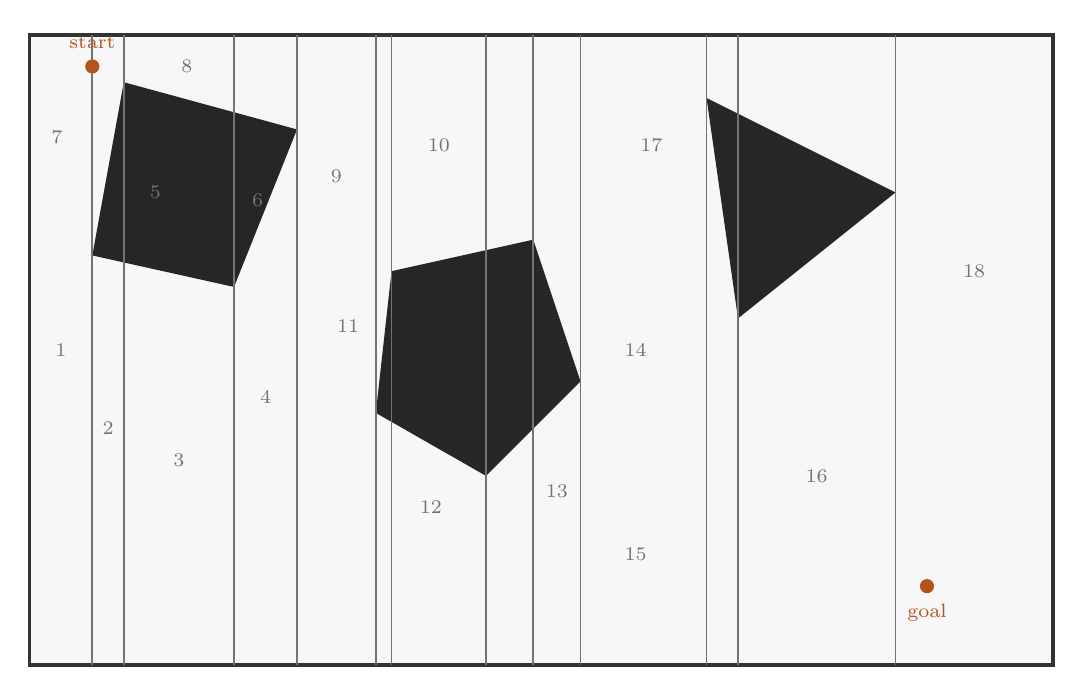
\begin{tikzpicture}[x=1cm,y=1cm]

  \draw[dbody, line width=1.2pt] (0,0) rectangle (13,8);

  % Obstáculo A: seta/dardo (superior-esquerda)
  \fill[black!85] (1.2,7.4) -- (3.4,6.8) -- (2.6,4.8) -- (0.8,5.2) -- cycle;
  % Obstáculo B: pentágono (centro)
  \fill[black!85] (4.6,5.0) -- (6.4,5.4) -- (7.0,3.6) -- (5.8,2.4) -- (4.4,3.2) -- cycle;
  % Obstáculo C: triângulo (superior-direita)
  \fill[black!85] (8.6,7.2) -- (11.0,6.0) -- (9.0,4.4) -- cycle;

  % Segmentos verticais erguidos em cada vértice
  \foreach \x in {0.8,1.2,2.6,3.4,4.4,4.6,5.8,6.4,7.0,8.6,9.0,11.0} {
    \draw[black!55, line width=0.6pt] (\x,0) -- (\x,8);
  }

  \fill[dorange] (0.8,7.6) circle (0.09);
  \node[dorange, font=\scriptsize, anchor=south] at (0.8,7.7) {start};
  \fill[dorange] (11.4,1.0) circle (0.09);
  \node[dorange, font=\scriptsize, anchor=north] at (11.4,0.9) {goal};

  % Numeração das células (regiões livres)
  \node[dlbl, font=\scriptsize] at (0.4,4.0) {1};
  \node[dlbl, font=\scriptsize] at (1.0,3.0) {2};
  \node[dlbl, font=\scriptsize] at (1.9,2.6) {3};
  \node[dlbl, font=\scriptsize] at (3.0,3.4) {4};
  \node[dlbl, font=\scriptsize] at (1.6,6.0) {5};
  \node[dlbl, font=\scriptsize] at (2.0,7.6) {8};
  \node[dlbl, font=\scriptsize] at (2.9,5.9) {6};
  \node[dlbl, font=\scriptsize] at (3.9,6.2) {9};
  \node[dlbl, font=\scriptsize] at (5.2,6.6) {10};
  \node[dlbl, font=\scriptsize] at (4.05,4.3) {11};
  \node[dlbl, font=\scriptsize] at (5.1,2.0) {12};
  \node[dlbl, font=\scriptsize] at (6.7,2.2) {13};
  \node[dlbl, font=\scriptsize] at (7.7,4.0) {14};
  \node[dlbl, font=\scriptsize] at (7.7,1.4) {15};
  \node[dlbl, font=\scriptsize] at (7.9,6.6) {17};
  \node[dlbl, font=\scriptsize] at (12.0,5.0) {18};
  \node[dlbl, font=\scriptsize] at (10.0,2.4) {16};
  \node[dlbl, font=\scriptsize] at (0.35,6.7) {7};

\end{tikzpicture}
\end{document}
